\subsection{\secState{D}Rule-Based Mixed Head-On with Converging}\label{s:testRuleMixed}

\paragraph{Scenario:} Four \emph{UAS} are approaching an airway \emph{intersection} at the \emph{same time} from \emph{opposite direction} in \emph{controlled airspace} (over 500 feet Above Ground Level). Each \emph{UAS} have following \emph{Collision Hazards}:
\begin{enumerate}
	\item \emph{Head on Collision Hazard} - An UAS is approaching from opposite direction which invokes need to avoid \emph{Collision Point} actively

	\item \emph{Active Converging Collision Hazard} -  An UAS is approaching from the \emph{right side}, which gives him \emph{Right of the Way} and invokes the need to avoid \emph{Intruder} actively.

	\item \emph{Passive Converging Collision Hazard} - An UAS is approaching from the \emph{left side}, which gave us \emph{Right of the Way} and imposes an obligation of \emph{active avoidance} on other \emph{UAS}.
\end{enumerate}

\begin{note}
	Presented scenario is \emph{the worst possible situation} in current \emph{manned aviation ATM}. 
\end{note}

\noindent\emph{Mentioned Collision Hazards} must be addressed by \emph{UTM} service in the following manner:

\begin{enumerate}
	\item \emph{Each UAS} in particular \emph{Controlled Space} periodically sends synchronized \emph{Position Notification} messages (tab. \ref{tab:positionNotification}). 
	
	\item \emph{UTM} service receives \emph{Position Notifications} and manages \emph{Collision Cases} (tab. \ref{tab:collisionCase}) in \emph{Controlled Space}. 
	
	\item \emph{UTM} detects multiple \emph{Collision Cases} with \emph{Collision Points} in  the vicinity.
	
	\item \emph{UTM} service creates \emph{Virtual Roundabout} and implements \emph{Normative Directive} on all \emph{UAS} in the area.
\end{enumerate}

\noindent\emph{Mission parameters} for four UAS systems are defined in (tab. \ref{tab:missionSetupRuleBasedMixedScenario}).

\begin{table}[H]
	\centering
	\begin{tabular}{c||c|c||c}
		\multirow{2}{*}{UAS} &\multicolumn{2}{c||}{Position} & \multirow{2}{*}{$\mathscr{WP}_1$} \\\cline{2-3}
		  & $[x,y,z]$           & $[\theta,\varpi,\psi]$           & \\\hline\hline
		1 & $[0,20,0]^T $       & $[0^\circ,0^\circ,0^\circ]^T$    & $[45,20,0]^T$\\\hline 
		2 & $[40,20,0]^T $       & $[0^\circ,0^\circ,180^\circ]^T$    & $[-5,20,0]^T$\\\hline 
		3 & $[20,0,0]^T $       & $[0^\circ,0^\circ,90^\circ]^T$    & $[20,45,0]^T$\\\hline 
		4 & $[20,40,0]^T $       & $[0^\circ,0^\circ,-90^\circ]^T$  & $[45,20,0]^T$\\ 
	\end{tabular}
	\caption{Mission setup for \emph{rule-based mixed} scenario.}
	\label{tab:missionSetupRuleBasedMixedScenario}
\end{table}

\paragraph{Assumptions:} Following assumptions are valid for this test:

\begin{enumerate}
	\item \emph{Controlled Airspace Airworthiness} - UAS system is equipped with necessary controlled airspace equipment like ADS-B In/Out, Radar, Transponder, etc. Moreover, airworthy \emph{UAS} has capability to precisely follow \emph{UTM directives} (max. 5 $\%$ deviation).
	
	\item \emph{C2 (Command \& control) Link Established} - necessary for (UAS $\leftrightarrow$ UAS) and (UAS $\leftrightarrow$ UTM) communication. If \emph{C2} link is lost the \emph{UAS} will enter into \emph{Emergency avoidance mode}.
	
	\item \emph{Decision frame synchronization with UTM} - necessary in discrete C2 environment otherwise \emph{safety margins} needs to be \emph{bloated}.
	
	\item \emph{Every UAS have identical cruising speed} - simplification impacting \emph{UTM} service implementation. \emph{Obstacle Avoidance Framework} can comprehend various intruders speed, with proper \emph{UAS} directives.
\end{enumerate}

\paragraph{Main Goal:} Show possibility of \emph{Virtual Roundabout} invoked by \emph{UTM} directives where \emph{Obstacle Avoidance Framework based on Reach Sets} is used as a \emph{Navigation Module}.

\paragraph{Acceptance  Criteria:} Following criteria must be met:

\begin{enumerate}
	\item \emph{Well Clear Condition valid for every UAS} - Each \emph{UAS} must have \emph{minimal required distance} from \emph{other UAS} for all \emph{Virtual Roundabout} enforcement time.
	
	\item \emph{Fulfillment of UTM Directives} - Each UAS must stay in a \emph{Navigation mode} for all \emph{Virtual Roundabout} enforcement time. Each \emph{UAS} must stay on \emph{Virtual Roundabout} for the necessary time, before leaving for \emph{Original Navigation waypoint $\mathscr{WP}_1$}.
\end{enumerate}

\paragraph{Testing Setup:} The \emph{standard test setup} for each UAS defined in (tab. \ref{tab:testMovementOrientations}, \ref{tab:testUASBasicParameters}, \ref{tab:testNavigationGridBasic}, \ref{tab:testAvoidanceGridBasic}, \ref{tab:testUASColoring}) is used with following parameter override:
\begin{enumerate}
	\item \emph{Navigation grid - type} - \emph{ACAS-like} with \emph{horizontal enabled maneuvers}
\end{enumerate}

This \emph{configuration} is based on the assumption that every UAS is in \emph{controlled airspace} in \emph{FL450} (flight level 45000 feet Above Sea Level), without permission for a \emph{climb or descent maneuver}. The \emph{rule engine} is initialized in standard \emph{Rules of the air} configuration (fig. \ref{fig:RuleEngineInstanceLevels}).

There is \emph{UTM} service for given \emph{airspace cluster} calculating \emph{collision cases} (tab. \ref{tab:collisionCase}) based on incoming \emph{UAS position notifications} (tab. \ref{tab:positionNotification}).

\paragraph{Simulation Run:} Notable moments from the \emph{simulation run} (fig. \ref{fig:testCaseRuleBasedMixed}) are the following:

\begin{enumerate}
	\item \emph{Collision cases created} (fig. \ref{fig:ruleMultipleCollisionCasesCreated}) following events happen in this step:
	\begin{enumerate}[a.]
		\item Four \emph{UAS} are approaching airways intersection: \emph{UAS 1} (blue) from left, \emph{UAS 2} (cyan) from right, \emph{UAS 3} (green) from the bottom, \emph{UAS 4} (black) from the top.
		
		\item They are going to collide at point $[20,20,0]^T$ of \emph{Flight level} (elevation is 45, 000 feet Above Mean Sea Level).
		
		\item \emph{UTM service} notices future \emph{Collision Situations} and creates \emph{Collision Cases}.
		
		\item There are many \emph{Collision Cases} in the near vicinity. The \emph{Virtual Roundabout} is created with \emph{Safety margin} $15$ $m$.
		
		\item The \emph{UTM} service then sends a new \emph{Roundabout Directives} to involved \emph{UAS} systems.
		
		\item Each \emph{UAS} starts \emph{Roundabout Entry Maneuver} by correcting own  \emph{Heading} and \emph{Speed} (if its necessary).
	\end{enumerate}   
	
	\item \emph{Roundabout entry} (fig. \ref{fig:ruleMultipleRoundabountEntry}) - Each \emph{UAS} enters into \emph{Virtual Roundabout} while sending \emph{Roundabout Entrance Notification} to \emph{UTM service}.
	
	\item \emph{Roundabout leave} (fig. \ref{fig:ruleMultipleRoundaboutLeave})  following events happens in this step:
	\begin{enumerate}[a.]
		\item Each \emph{UAS} when is going to approach the level of \emph{Original Goal Waypoint} sends \emph{Roundabout Leave Request}.
		
		\item UTM system will check if there is \emph{Sufficient Free Space} to leave \emph{Virtual Roundabout}.
		
		\item The \emph{UTM Service then issues} \emph{Virtual Roundabout Leave Approval}.
		
		\item Each \emph{UAS} will correct own heading and speed in the range of received permit.
	\end{enumerate}   
	
	\item \emph{Situation resolution} (fig. \ref{fig:ruleMultipleSituationResolution}) - Each \emph{UAS} is heading away from \emph{Roundabout Center}, there is no active user of \emph{Virtual Roundabout}. \emph{UTM} will remove \emph{Virtual Roundabout}  and closes underlying \emph{Collision Cases}. Each \emph{UAS} will reach respective \emph{Original Goal Waypoint}.
\end{enumerate}


\begin{figure}[H]
	\centering
	\begin{subfigure}{0.48\textwidth}
		\centering
		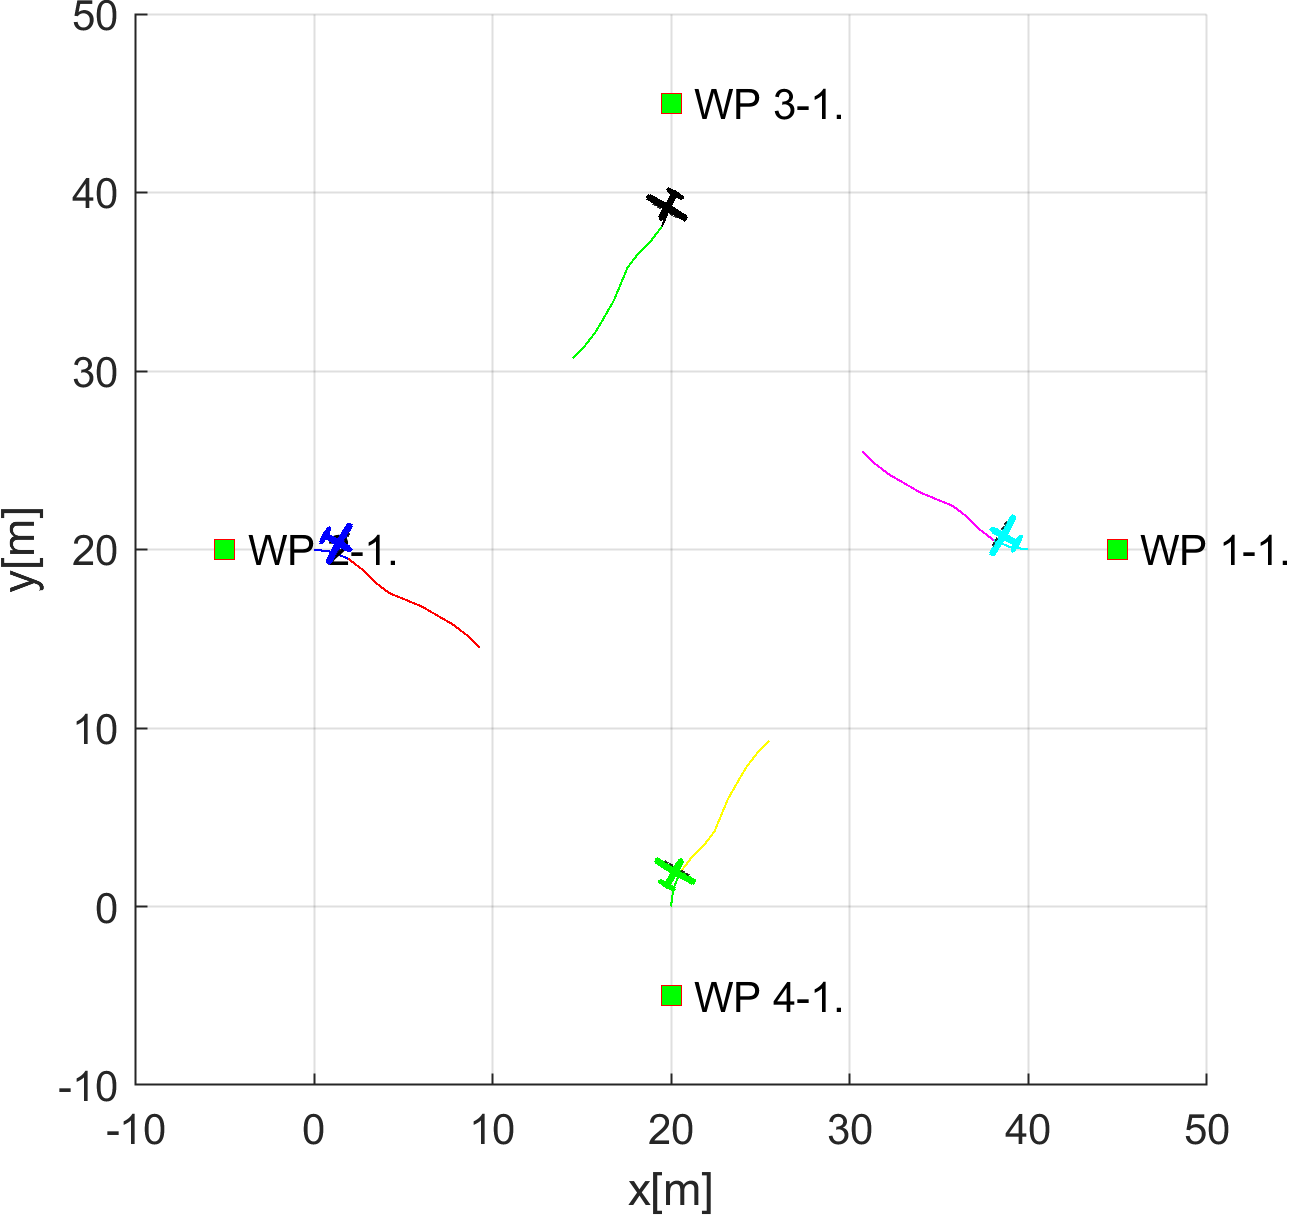
\includegraphics[width=0.9\linewidth]{\FIGDIR/NS062UtmCooperativeHeadOnMultiple00002}
		\caption{Collision cases created.}
		\label{fig:ruleMultipleCollisionCasesCreated}
	\end{subfigure}
	\begin{subfigure}{0.48\textwidth}
		\centering
		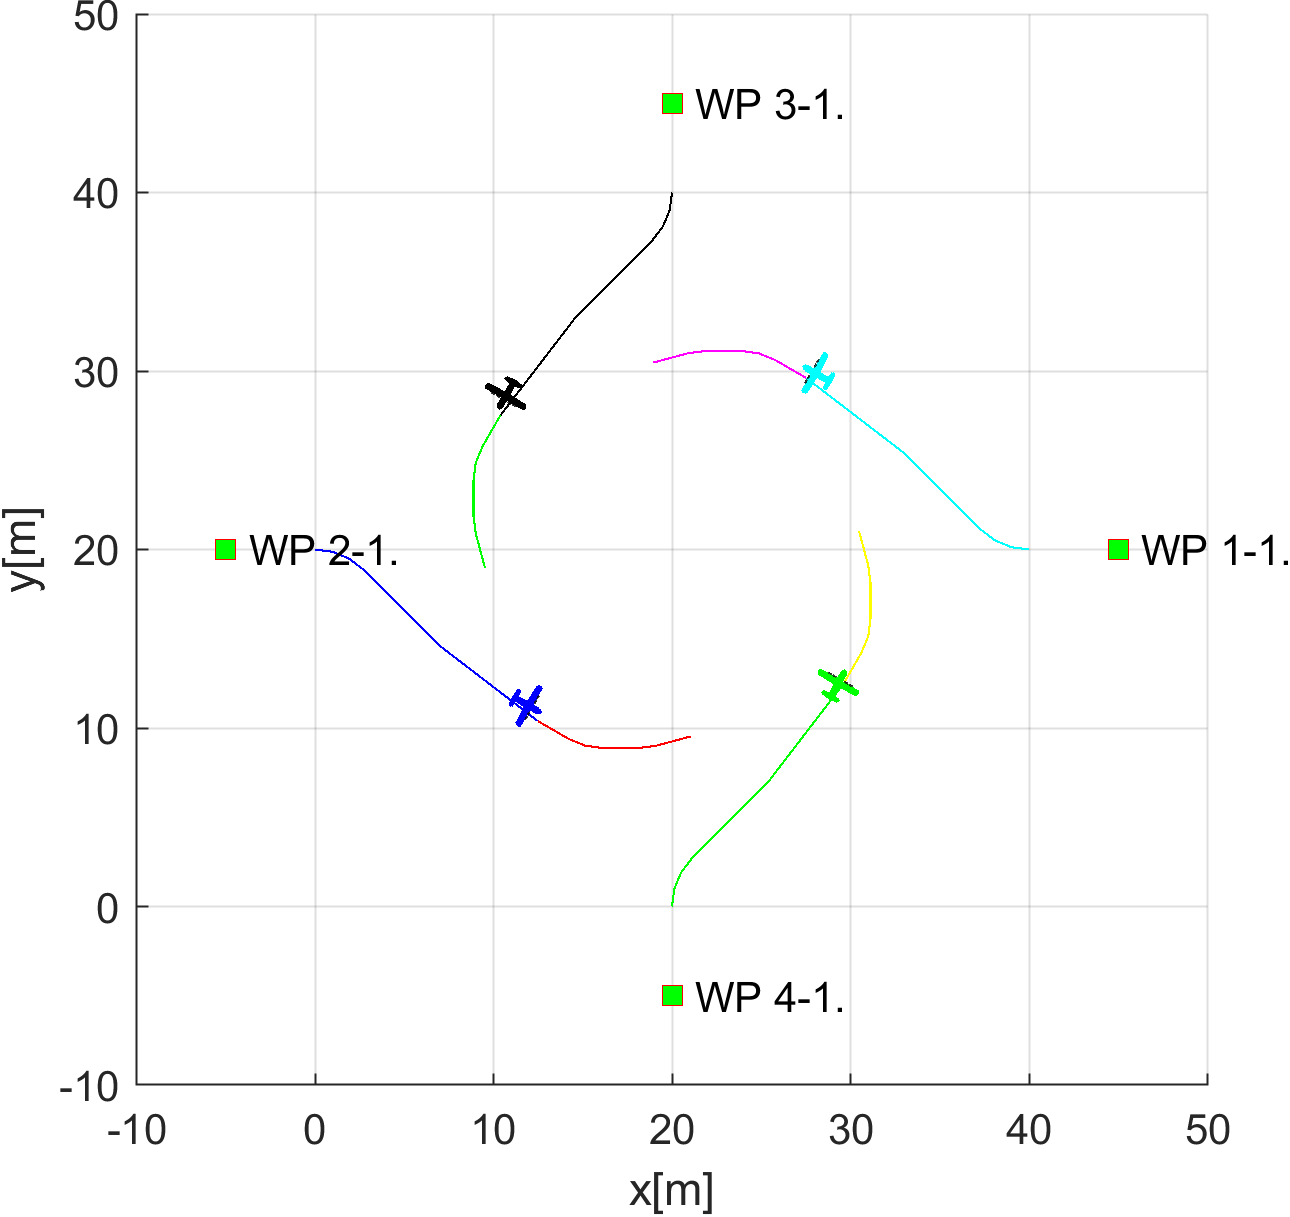
\includegraphics[width=0.9\linewidth]{\FIGDIR/NS063UtmCooperativeHeadOnMultiple00016} 
		\caption{Roundabout entry.}
		\label{fig:ruleMultipleRoundabountEntry}
	\end{subfigure}
	\\
	\begin{subfigure}{0.48\textwidth}
		\centering
		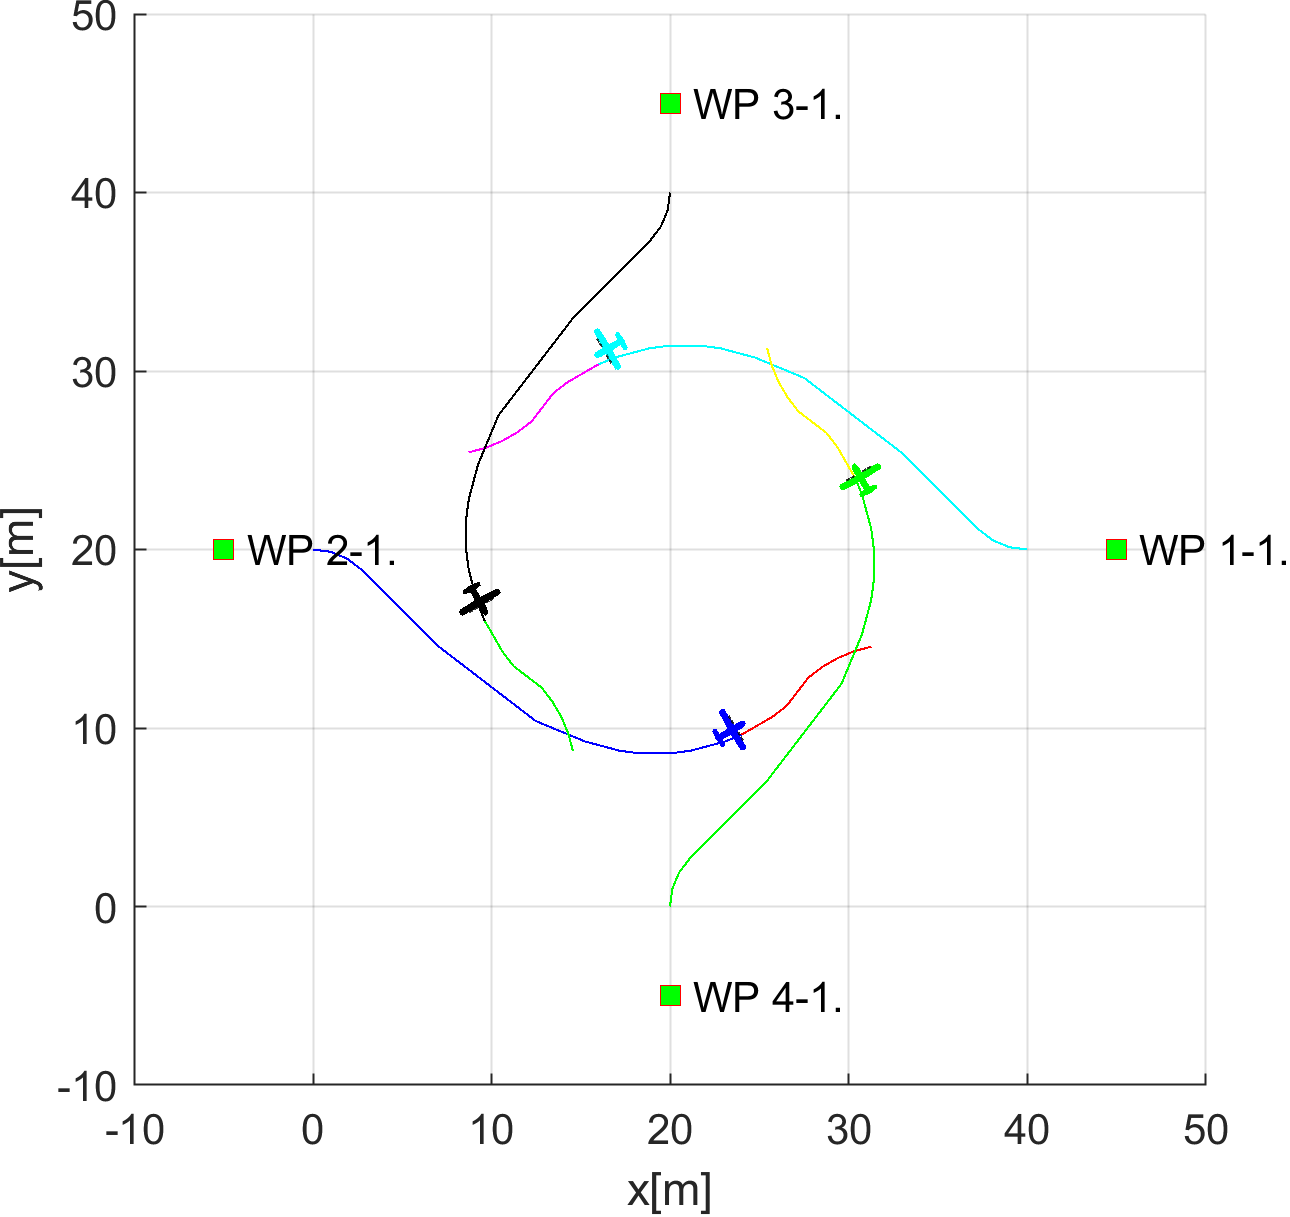
\includegraphics[width=0.9\linewidth]{\FIGDIR/NS064UtmCooperativeHeadOnMultiple00028} 
		\caption{Roundabout leave.}
		\label{fig:ruleMultipleRoundaboutLeave}
	\end{subfigure}
	\begin{subfigure}{0.48\textwidth}
		\centering
		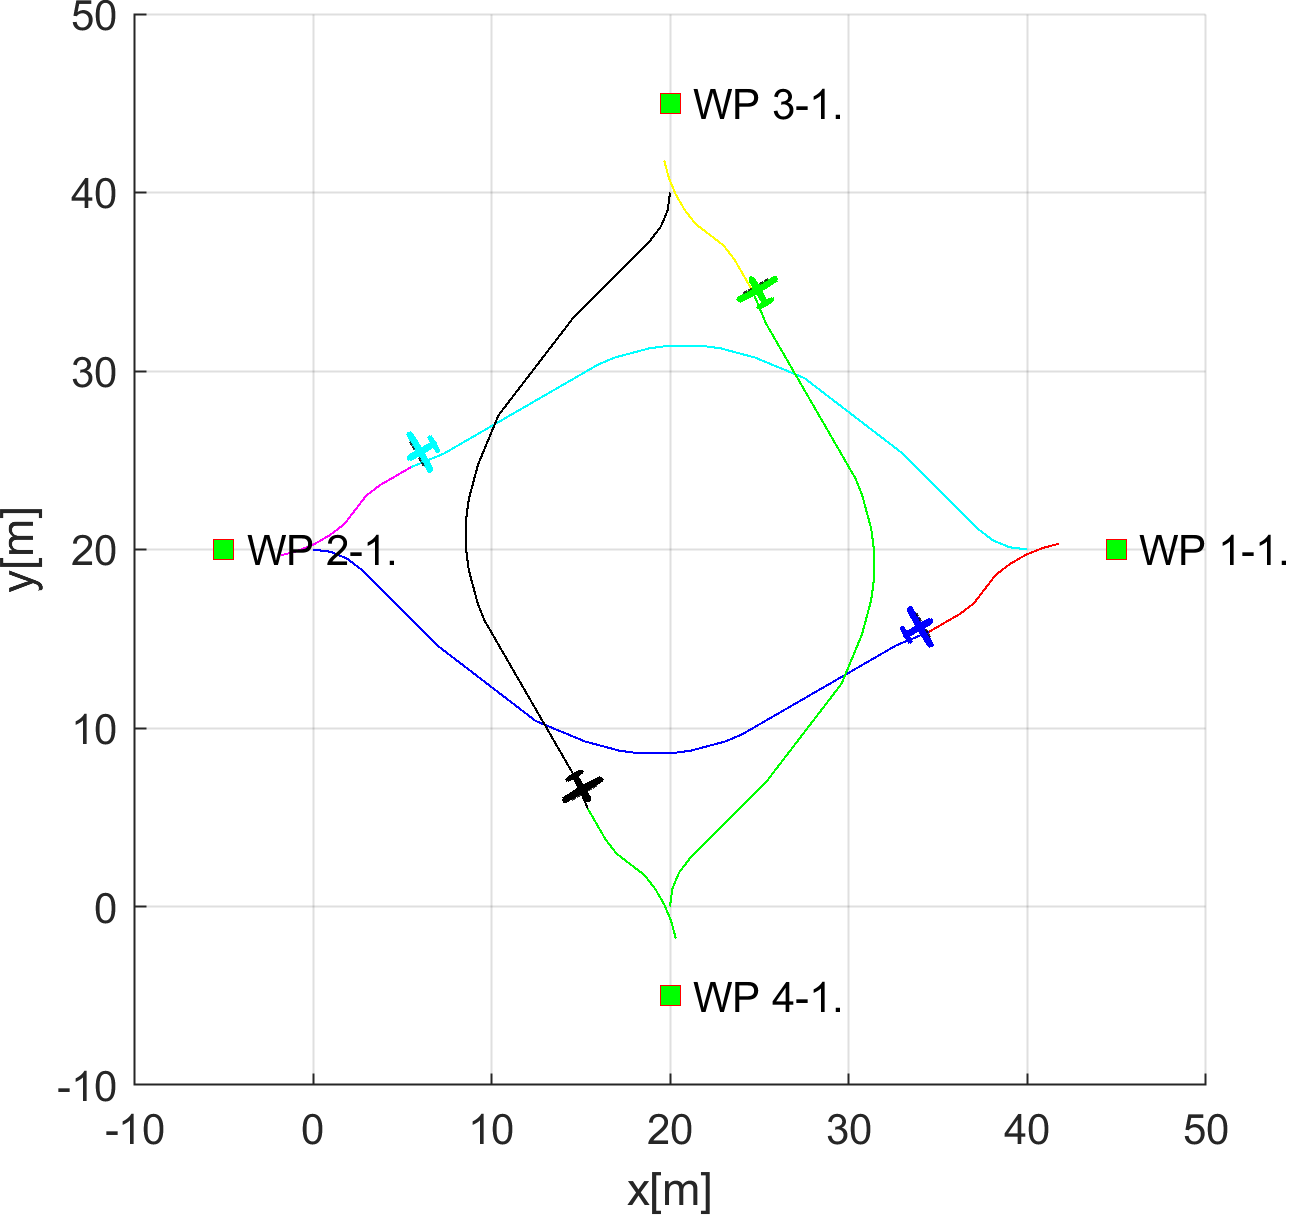
\includegraphics[width=0.9\linewidth]{\FIGDIR/NS065UtmCooperativeHeadOnMultiple00040} 
		\caption{Situation resolution.}
		\label{fig:ruleMultipleSituationResolution}
	\end{subfigure}
	\caption{Test scenario for \emph{rule-based mixed} situation with the \emph{self-separation mode}.}
	\label{fig:testCaseRuleBasedMixed}
\end{figure}

\paragraph{Collision Cases Calculation:} The set of original \emph{Collision cases} is given in (tab. \ref{tab:collisionCasesRuleBasedMixed}). 

Each \emph{UAS} has one \emph{Head on}, \emph{Converging passive}, \emph{Converging active} collision hazard. For example \emph{UAS 1} have a \emph{head-on} with  \emph{UAS 2}, \emph{converging passive} with \emph{UAS 4}, \emph{converging active} with \emph{UAS 3}. For \emph{UAS 2-4} check \emph{role} in respective \emph{Collision Cases}.

\begin{note} \emph{Collision cases} calculated by \emph{UTM} are symmetric, which means that collision case for \emph{UAS X, UAS Y} is identical to collision case calculated for \emph{UAS Y, UAS X}, $X \neq Y$.
\end{note}

\emph{Safety margin} representing \emph{Well Clear Margin} for single \emph{UAS} in \emph{Collision Case} ranges $5-8$ $m$. \emph{Case margin} representing the minimal mutual distance between two \emph{UAS systems} to remain well clear ranges $12-15$ $m$.

\emph{Merged Collision Case} is oversimplified for demonstration purposes. \emph{Merge Case Procedure} is out of the scope of this work due to its extent. Every \emph{Collision Case} shares same \emph{Collision Point} $[20,20,0]^T$ in flight level coordinate frame. \emph{Merged Collision Case} type was set as \emph{Roundabout}, due the number of collision case \emph{attendants} is greater than 2. Each \emph{UAS role} has been set as \emph{Roundabout}. The enforced \emph{safety margin} is equal to $15$ $m$, which is the maximum of all \emph{single collision case combined margins}.

\begin{table}[H]
	\centering
	\begin{tabular}{c|c|c|c|c|c||c|c}
		\multicolumn{6}{c||}{Collision Case}& \multicolumn{2}{c}{Margins} \\ \hline
		id  & UAS & role & \begin{tabular}[c]{@{}c@{}}collision\\ point\end{tabular} & \begin{tabular}[c]{@{}c@{}}angle of\\ approach\end{tabular} & type&  safety  & case  \\ \hline\hline
		% Case 1-2
		\multirow{2}{*}{1-2} & 1   & Roundabout & \multirow{2}{*}{$[20,20,0]^T$} & \multirow{2}{*}{$180^\circ$} & \multirow{2}{*}{Head on} & 8 & \multirow{2}{*}{15} \\ \cline{2-3} \cline{7-7} & 2   & Roundabout & & & & 7& \\ \hline
		% Case 1-3
		\multirow{2}{*}{1-3} & 1   & Converging & \multirow{2}{*}{$[20,20,0]^T$} & \multirow{2}{*}{$90^\circ$} & \multirow{2}{*}{Converging} & 8 & \multirow{2}{*}{15} \\ \cline{2-3} \cline{7-7} & 3   & Right o.W. & & & & 5& \\ \hline
		% Case 1-4
		\multirow{2}{*}{1-4} & 1   & Right o.W. & \multirow{2}{*}{$[20,20,0]^T$} & \multirow{2}{*}{$90^\circ$} & \multirow{2}{*}{Converging} & 8 & \multirow{2}{*}{15} \\ \cline{2-3} \cline{7-7} & 4   & Converging & & & & 5& \\ \hline
		% Case 2-3
		\multirow{2}{*}{2-3} & 2   & Right o.W. & \multirow{2}{*}{$[20,20,0]^T$} & \multirow{2}{*}{$90^\circ$} & \multirow{2}{*}{Converging} & 7 & \multirow{2}{*}{12} \\ \cline{2-3} \cline{7-7} & 3   & Converging & & & & 5& \\ \hline
		% Case 2-4
		\multirow{2}{*}{2-4} & 2   & Converging & \multirow{2}{*}{$[20,20,0]^T$} & \multirow{2}{*}{$90^\circ$} & \multirow{2}{*}{Converging} & 7 & \multirow{2}{*}{12} \\ \cline{2-3} \cline{7-7} & 4   & Right o.W. & & & & 5& \\ \hline
		% Case 3-4
		\multirow{2}{*}{3-4} & 3   & Roundabout & \multirow{2}{*}{$[20,20,0]^T$} & \multirow{2}{*}{$180^\circ$} & \multirow{2}{*}{Head on} & 7 & \multirow{2}{*}{14} \\ \cline{2-3} \cline{7-7} & 4   & Roundabout & & & & 7& \\\hline\hline
		% Merged case - header 
		\multicolumn{6}{c||}{Merged cases} & \multicolumn{2}{c}{\multirow{2}{*}{\begin{tabular}[c]{@{}c@{}}  Safety \\ Margin\end{tabular}}} \\ \cline{1-6} 
		id & UAS & role & \multicolumn{2}{c|}{collision point} & type& \multicolumn{2}{c}{} \\ \hline\hline
		% line 1
		\multirow{4}{*}{\begin{tabular}[c]{@{}c@{}}1-2-\\ -3-4\end{tabular}} & 1   & Roundabout & \multicolumn{2}{c|}{\multirow{4}{*}{$[20,20,0]^T$}} & \multirow{4}{*}{Roundabout} & \multicolumn{2}{c}{\multirow{4}{*}{15}} \\ \cline{2-3}
		% line 2
		& 2   & Roundabout & \multicolumn{2}{c|}{} & & \multicolumn{2}{c}{}\\ \cline{2-3}
		% line 3
		& 3   & Roundabout & \multicolumn{2}{c|}{} & & \multicolumn{2}{c}{}\\ \cline{2-3}
		% line 4
		& 4   & Roundabout & \multicolumn{2}{c|}{} & & \multicolumn{2}{c}{}\\ 
	\end{tabular}
	\caption{Collision cases for \emph{rule-based mixed} scenario.}
	\label{tab:collisionCasesRuleBasedMixed}
\end{table}

\paragraph{Distance to Safety Margin Evolution:} \emph{Merged Collision Case Safety Margin} is $15$ $m$, and it is valid for all \emph{UAS mutual distances}. The simple condition for \emph{Remain Well Clear} is:

\begin{equation*}
	crashDistance(UAS_X,UAS_Y,t) \ge 15 m, X\neq Y \in \{1,2,3,4\}, t\in utmTime
\end{equation*}

\noindent \emph{Safety Margin Performance} is given in (fig. \ref{fig:testRuleBasedMultipleAvoidancePerformance}). The mutual distance (Crash Distance [m]) between two UAS is denoted as the \emph{blue line}. The enforced safety margin for \emph{Remain Well Clear} condition is denoted as the red line.

\begin{note}
	\emph{Evolution of mutual crash distance} is symmetric. In any case, the mutual distance goes under \emph{safety margin}. \emph{Acceptance criterion} for \emph{Well Clear condition} is fulfilled.
\end{note}
	
\begin{figure}[H]
	\centering
	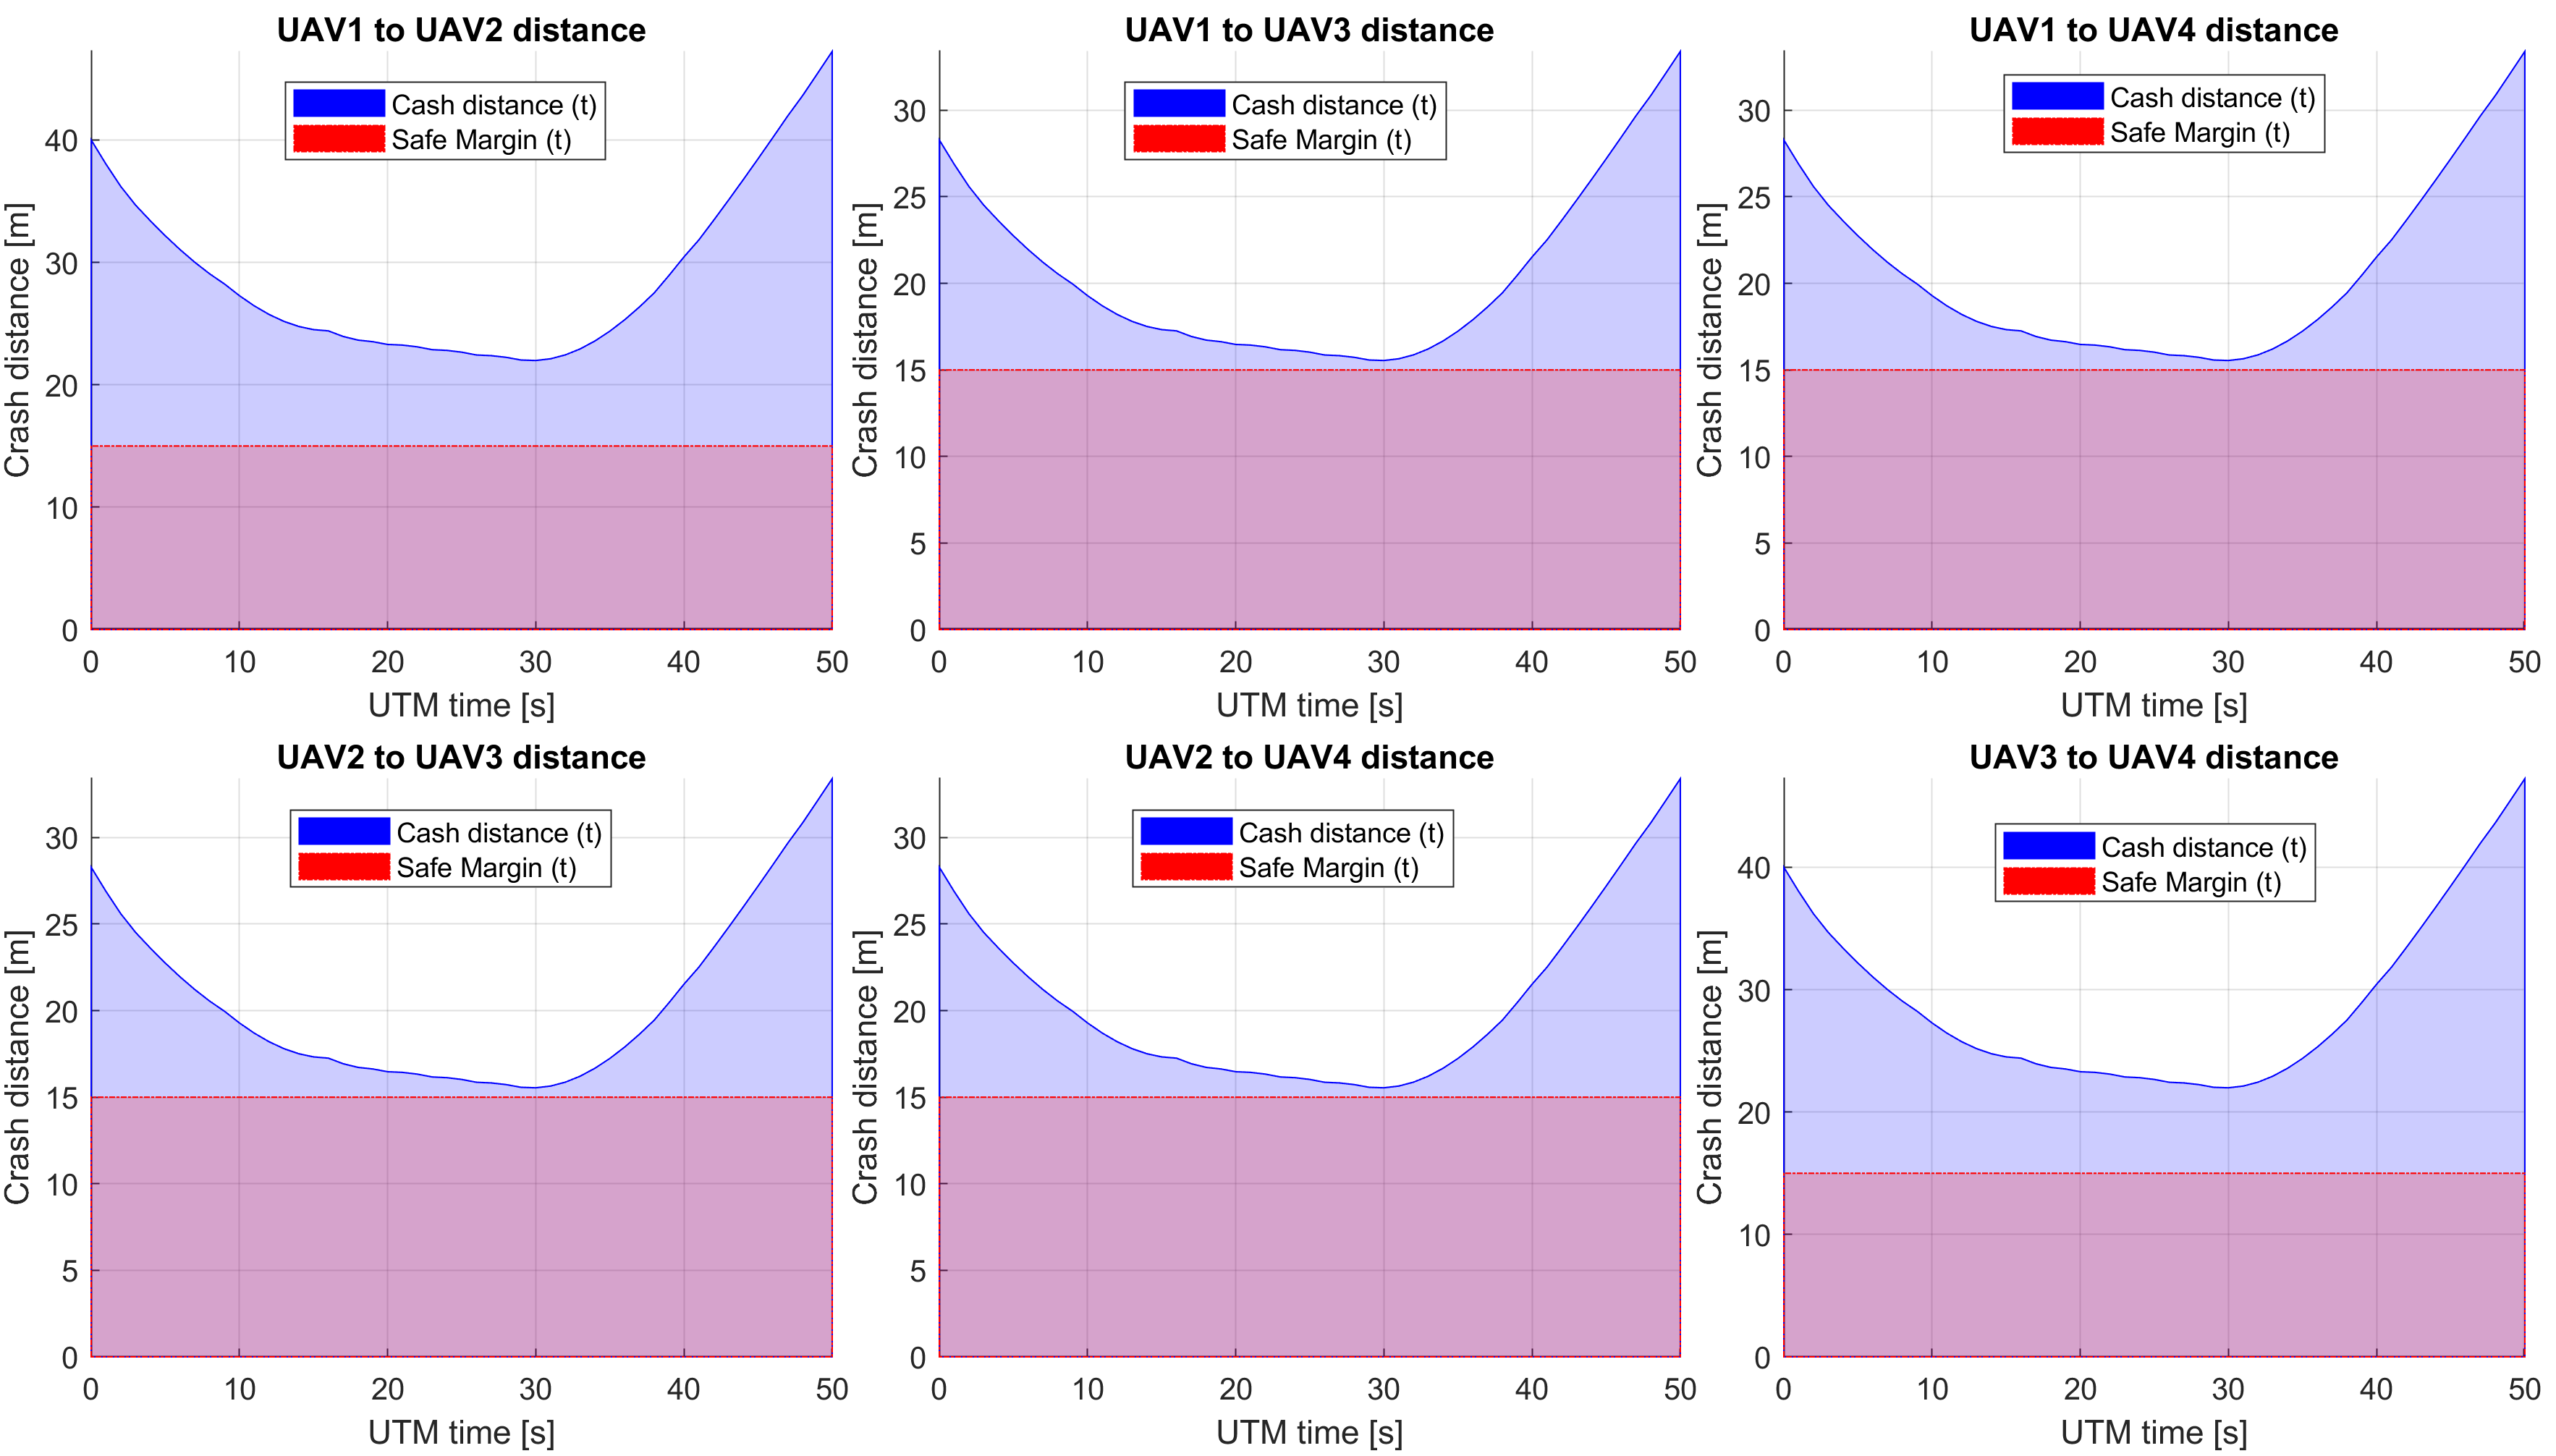
\includegraphics[width=0.9\linewidth]{\FIGDIR/NS066UtmCooperativeHeadOnMultiplePerformance}
	\caption{Distance to safety margin evolution for \emph{rule-based mixed scenario}.}
	\label{fig:testRuleBasedMultipleAvoidancePerformance}
\end{figure}

\paragraph{Distance to Safety Margin Peaks:} \emph{Distance to Safety Margin Peaks} (tab. \ref{tab:testCaseRuleBasedMixedSafetyMarginDistances}) represents the proximity of \emph{UAS mutual distance to breach well clear condition}. The \emph{breach condition} was not fulfilled in any combination. 

The \emph{minimal distance to safety margin} was $0.5438$ $m$ between all four \emph{UAS} systems. The \emph{maximal distance to safety margin} ranges between \emph{18 - 32 m} which show advantages of the \emph{virtual roundabout}.

\begin{table}[H]
	\centering
	\begin{tabular}{c||c|c|c}
		\multirow{2}{*}{UAS:} & \multicolumn{3}{c}{Distance to Safety Margin} \\ \cline{2-4} 
				  & min          & max         & breach         \\ \hline\hline
			1-2   & 6.9823       & 32.2369     & false          \\ \hline
			1-3   & 0.5438       & 18.4015     & false          \\ \hline
			1-4   & 0.5438       & 18.4015     & false          \\ \hline
			2-3   & 0.5438       & 18.4015     & false          \\ \hline
			2-4   & 0.5438       & 18.4015     & false          \\ \hline
			3-4   & 6.9823       & 32.2369     & false          \\ 
	\end{tabular}
	\caption{Distance to safety margin peaks for \emph{rule-based mixed scenario}.}
	\label{tab:testCaseRuleBasedMixedSafetyMarginDistances}
\end{table}


\paragraph{Path Tracking Performance:} Path tracking is displayed in (fig. \ref{fig:testCaseRuleBasedMixedTrajectoryTracking}). The UAS trajectory is divided into \emph{X, Y, Z axis tracking over UTM Time}. The \emph{Reference Trajectory} (green dashed line) is represented as the interconnection between \emph{Start Waypoint} (green square marked S) and  \emph{Goal Waypoint $\mathscr{WP}_1$} (green square marked 1). The \emph{Executed trajectory} (solid blue  line) reflects real \emph{UAS} movement.

\begin{enumerate}
	\item \emph{UAS 1} (fig. \ref{fig:ruleBasedMixedPathTrackingUAS1}) is using the bottom portion of \emph{Virtual Roundabout} (-Y values), sticking to the boundary of the \emph{Virtual Roundabout}.
	
	\item \emph{UAS 2} (fig. \ref{fig:ruleBasedMixedPathTrackingUAS2}) is using the upper portion of the \emph{Virtual Roundabout}. (+Y values), sticking to the boundary of the \emph{Virtual Roundabout}.
	
	\item \emph{UAS 3} (fig. \ref{fig:ruleBasedMixedPathTrackingUAS3}) is using the right portion of the \emph{Virtual Roundabout}. (+X values), sticking to the boundary of the \emph{Virtual Roundabout}.
	
	\item \emph{UAS 4} (fig. \ref{fig:ruleBasedMixedPathTrackingUAS4}) is using the left portion of the \emph{Virtual Roundabout}. (-X values), sticking to the boundary of the \emph{Virtual Roundabout}.
\end{enumerate}

\begin{figure}[H]
	\centering
	\begin{subfigure}{0.48\textwidth}
		\centering
		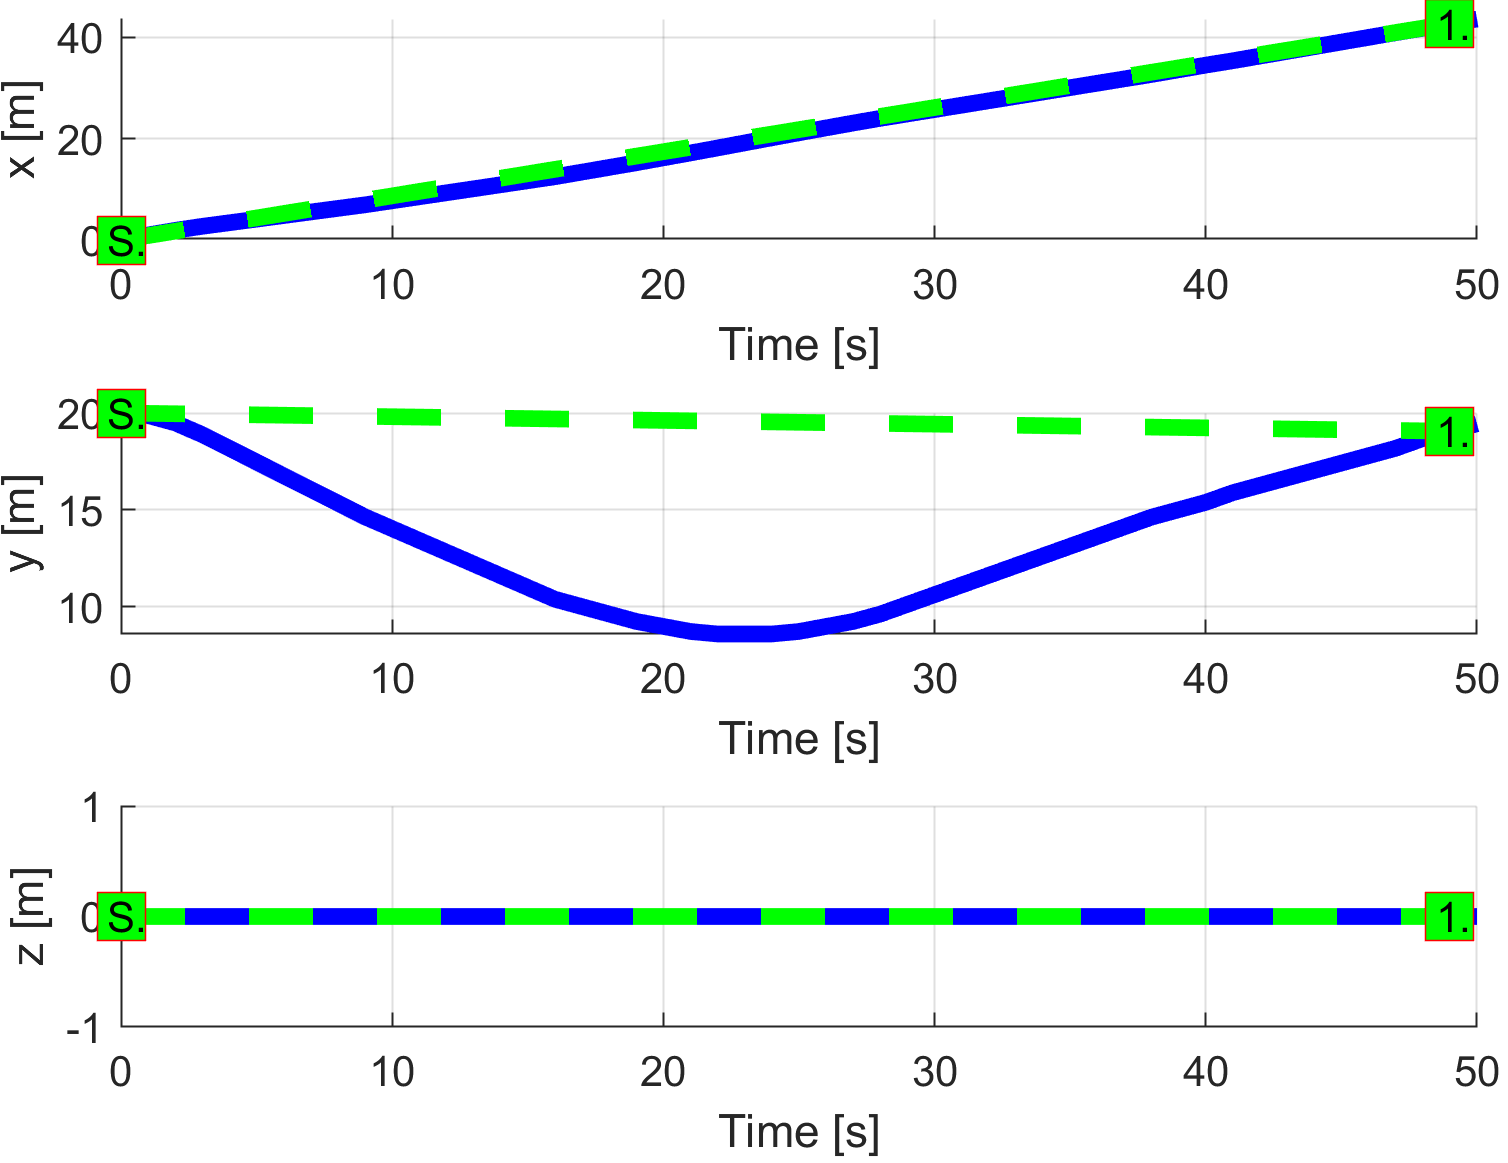
\includegraphics[width=0.9\linewidth]{\FIGDIR/NS067UtmCooperativeHeadOnMultipleUAV1PathFollowing}
		\caption{UAS 1.}
		\label{fig:ruleBasedMixedPathTrackingUAS1}
	\end{subfigure}
	\begin{subfigure}{0.48\textwidth}
		\centering
		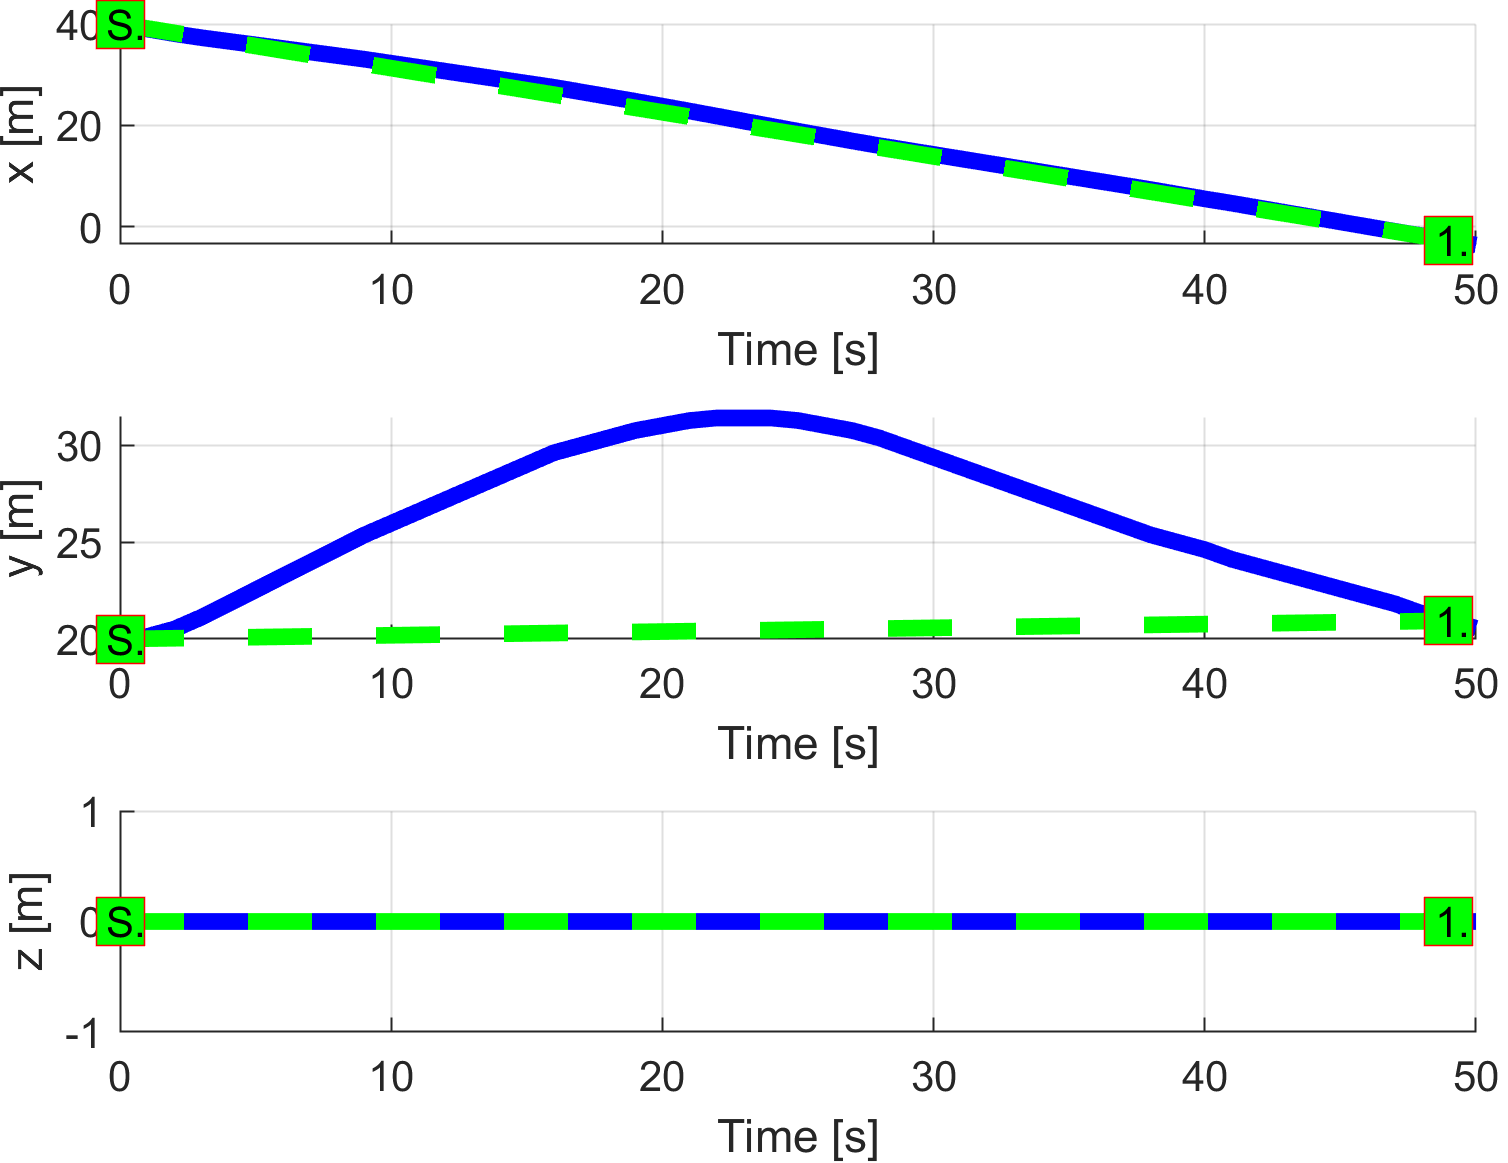
\includegraphics[width=0.9\linewidth]{\FIGDIR/NS068UtmCooperativeHeadOnMultipleUAV2PathFollowing} 
		\caption{UAS 2.}
		\label{fig:ruleBasedMixedPathTrackingUAS2}
	\end{subfigure}
	\\
	\begin{subfigure}{0.48\textwidth}
		\centering
		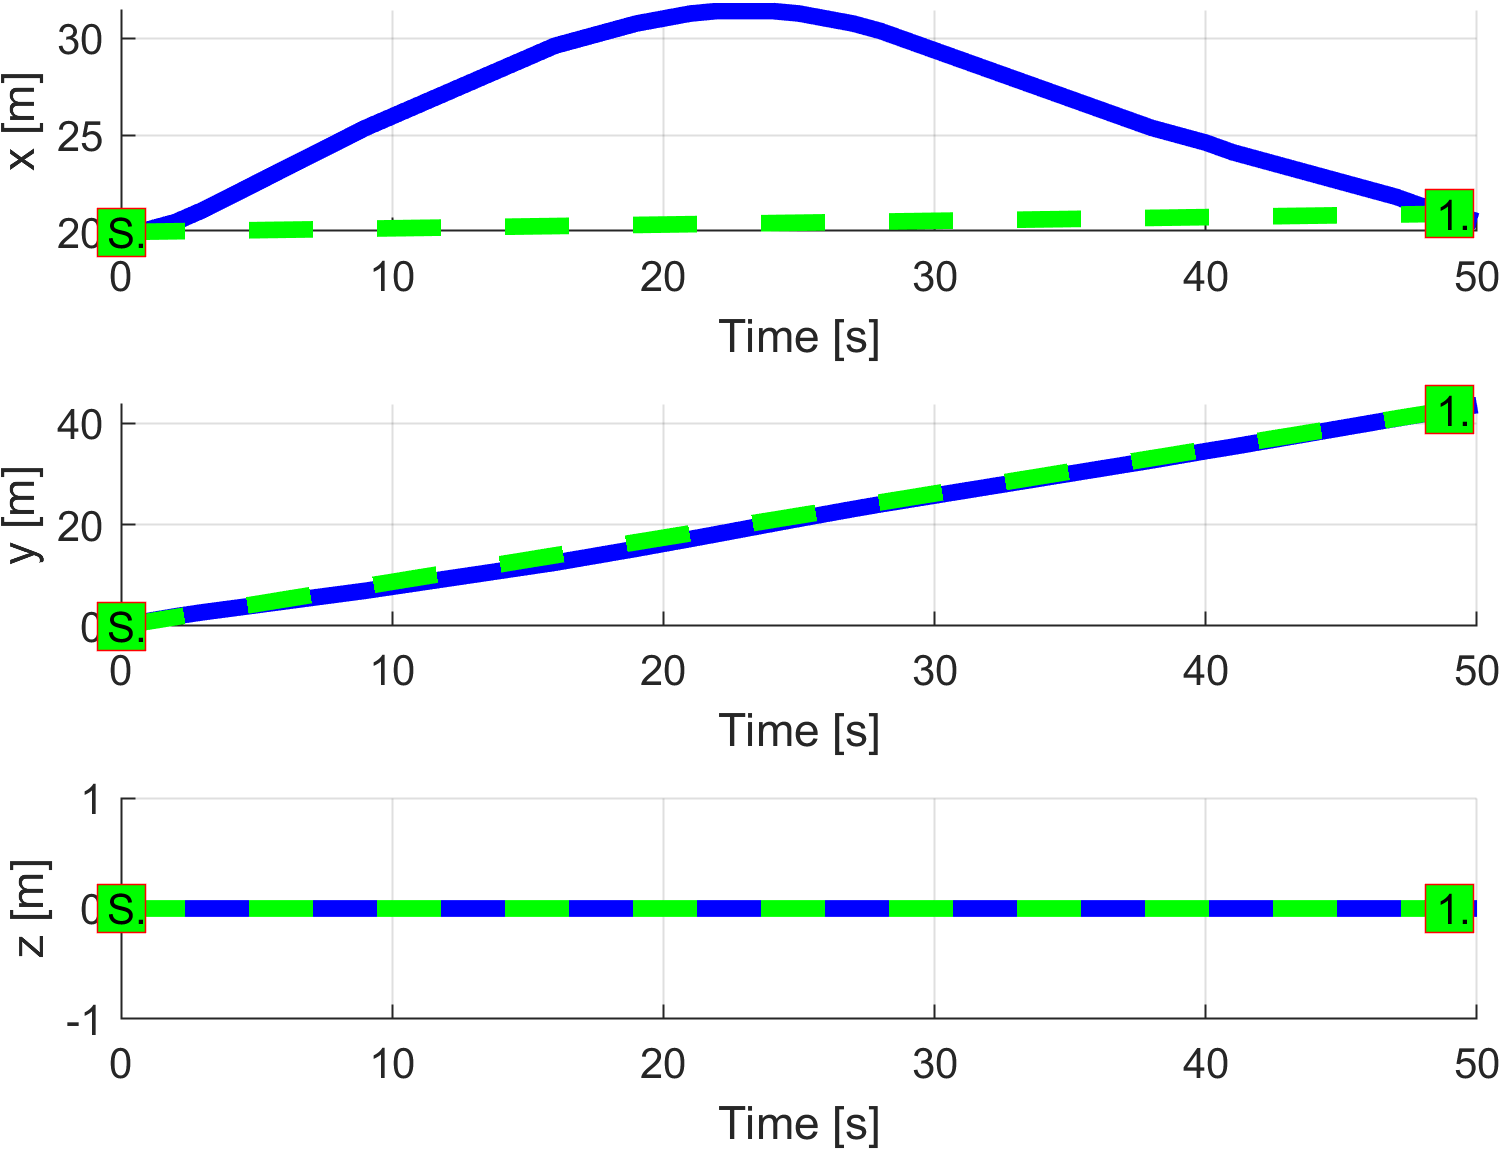
\includegraphics[width=0.9\linewidth]{\FIGDIR/NS069UtmCooperativeHeadOnMultipleUAV3PathFollowing} 
		\caption{UAS 3.}
		\label{fig:ruleBasedMixedPathTrackingUAS3}
	\end{subfigure}
	\begin{subfigure}{0.48\textwidth}
		\centering
		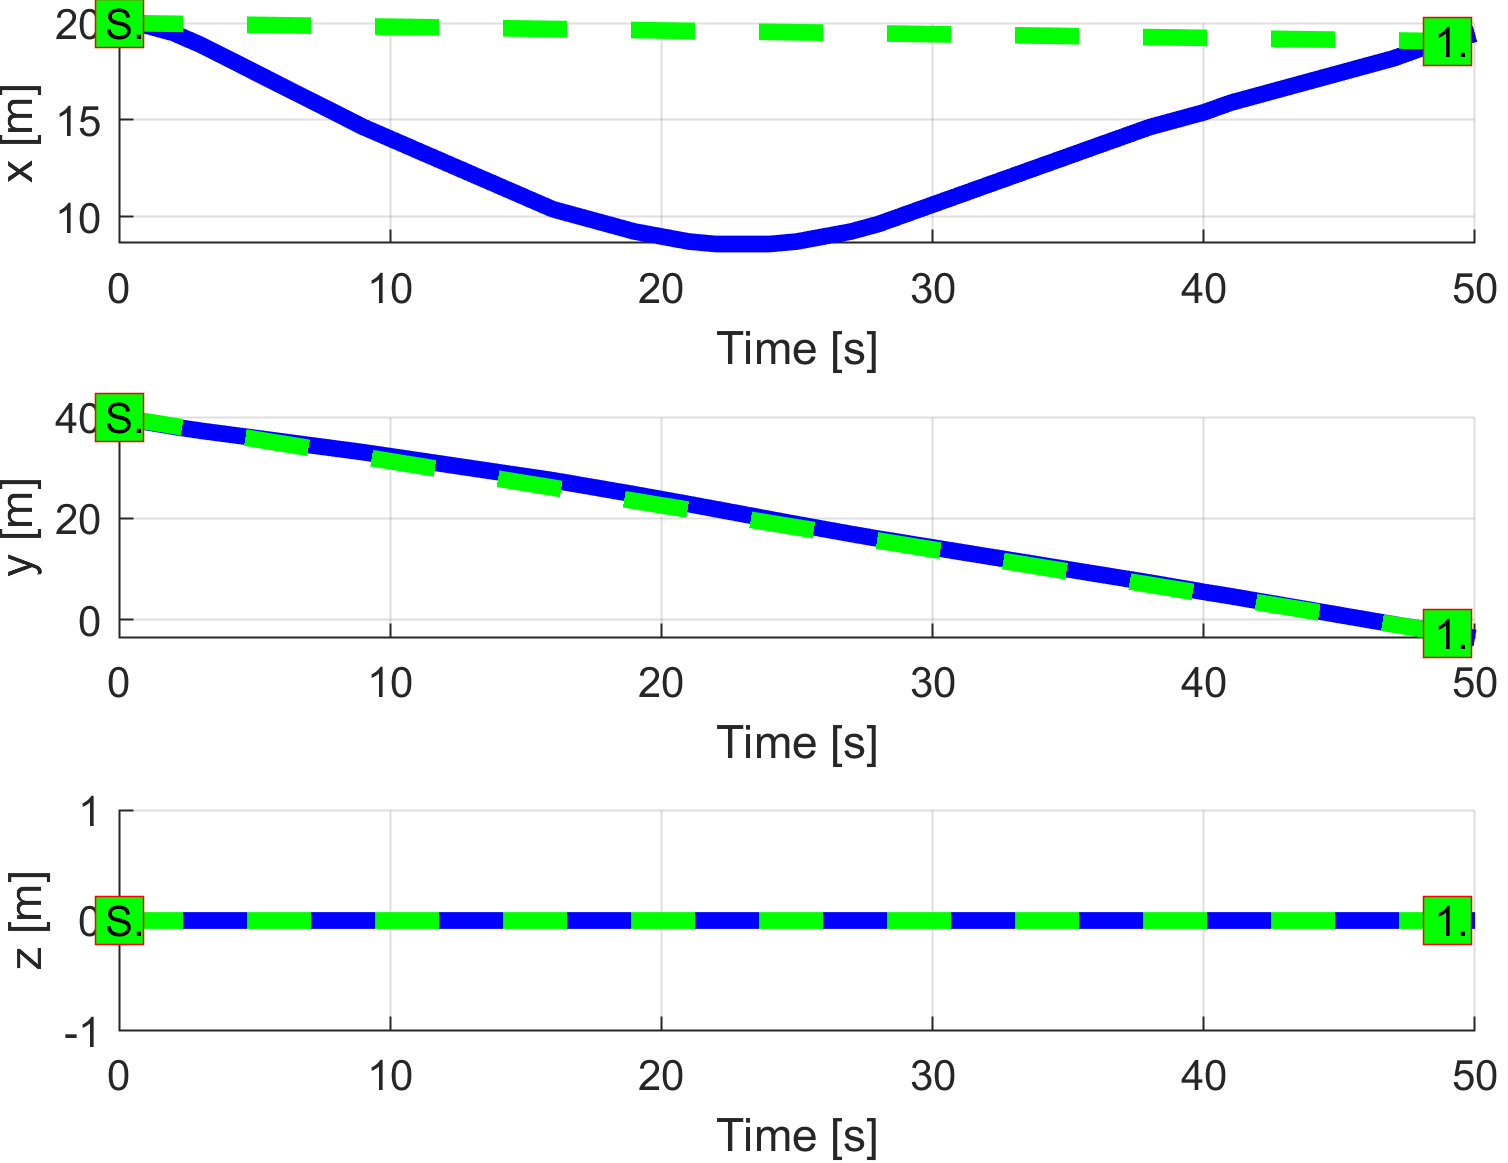
\includegraphics[width=0.9\linewidth]{\FIGDIR/NS070UtmCooperativeHeadOnMultipleUAV4PathFollowing} 
		\caption{UAS 4.}
		\label{fig:ruleBasedMixedPathTrackingUAS4}
	\end{subfigure}
	\caption{Trajectory tracking for \emph{rule-based mixed} situation test case.}
	\label{fig:testCaseRuleBasedMixedTrajectoryTracking}
\end{figure}

\paragraph{Path Tracking Deviations:} \emph{Deviations} (tab. \ref{tab:pathTrackingParametersForRuleBasedMixed}) are in expected ranges, considering the mission plans (tab. \ref{tab:missionSetupRuleBasedMixedScenario}) and \emph{Merged Case Safety Margin} ($15$ $m$).

\begin{table}[H]
	\centering
	\begin{tabular}{c||c|c|c|c}
		\multirow{2}{*}{Param.} & UAS 1     & UAS 2             & UAS 3             & UAS 4 \\\cline{2-5}
						& $\mathscr{WP}_1$  & $\mathscr{WP}_1$  & $\mathscr{WP}_1$  & $\mathscr{WP}_1$ \\\hline\hline
		  $\max |x|$    & 0                 & 0                 & 11.40             & 11.40\\\hline
		  $\max |y|$    & 11.40             & 11.40             & 0                 & 0\\\hline
		  $\max |z|$    & 0                 & 0                 & 0                 & 0\\\hline
		  $\max dist.$  & 11.40             & 11.40             & 11.40              & 11.40\\
	\end{tabular}
	\caption{Path tracking properties for \emph{rule-based mixed} scenario.}
	\label{tab:pathTrackingParametersForRuleBasedMixed}
\end{table}


% 10 Rule Based Multiple
\paragraph{Computation Load:} The \emph{computation load} for \emph{scenario} (fig.\ref{fig:ruleBasedMultipleComputationTime}) shows used time (y-axis) over decision frame (x-axis).

The \emph{computation time} for each UAS has the same evolution. The \emph{load} is higher  during avoidance maneuver on the \emph{virtual roundabout}.

\begin{figure}[H]
\centering
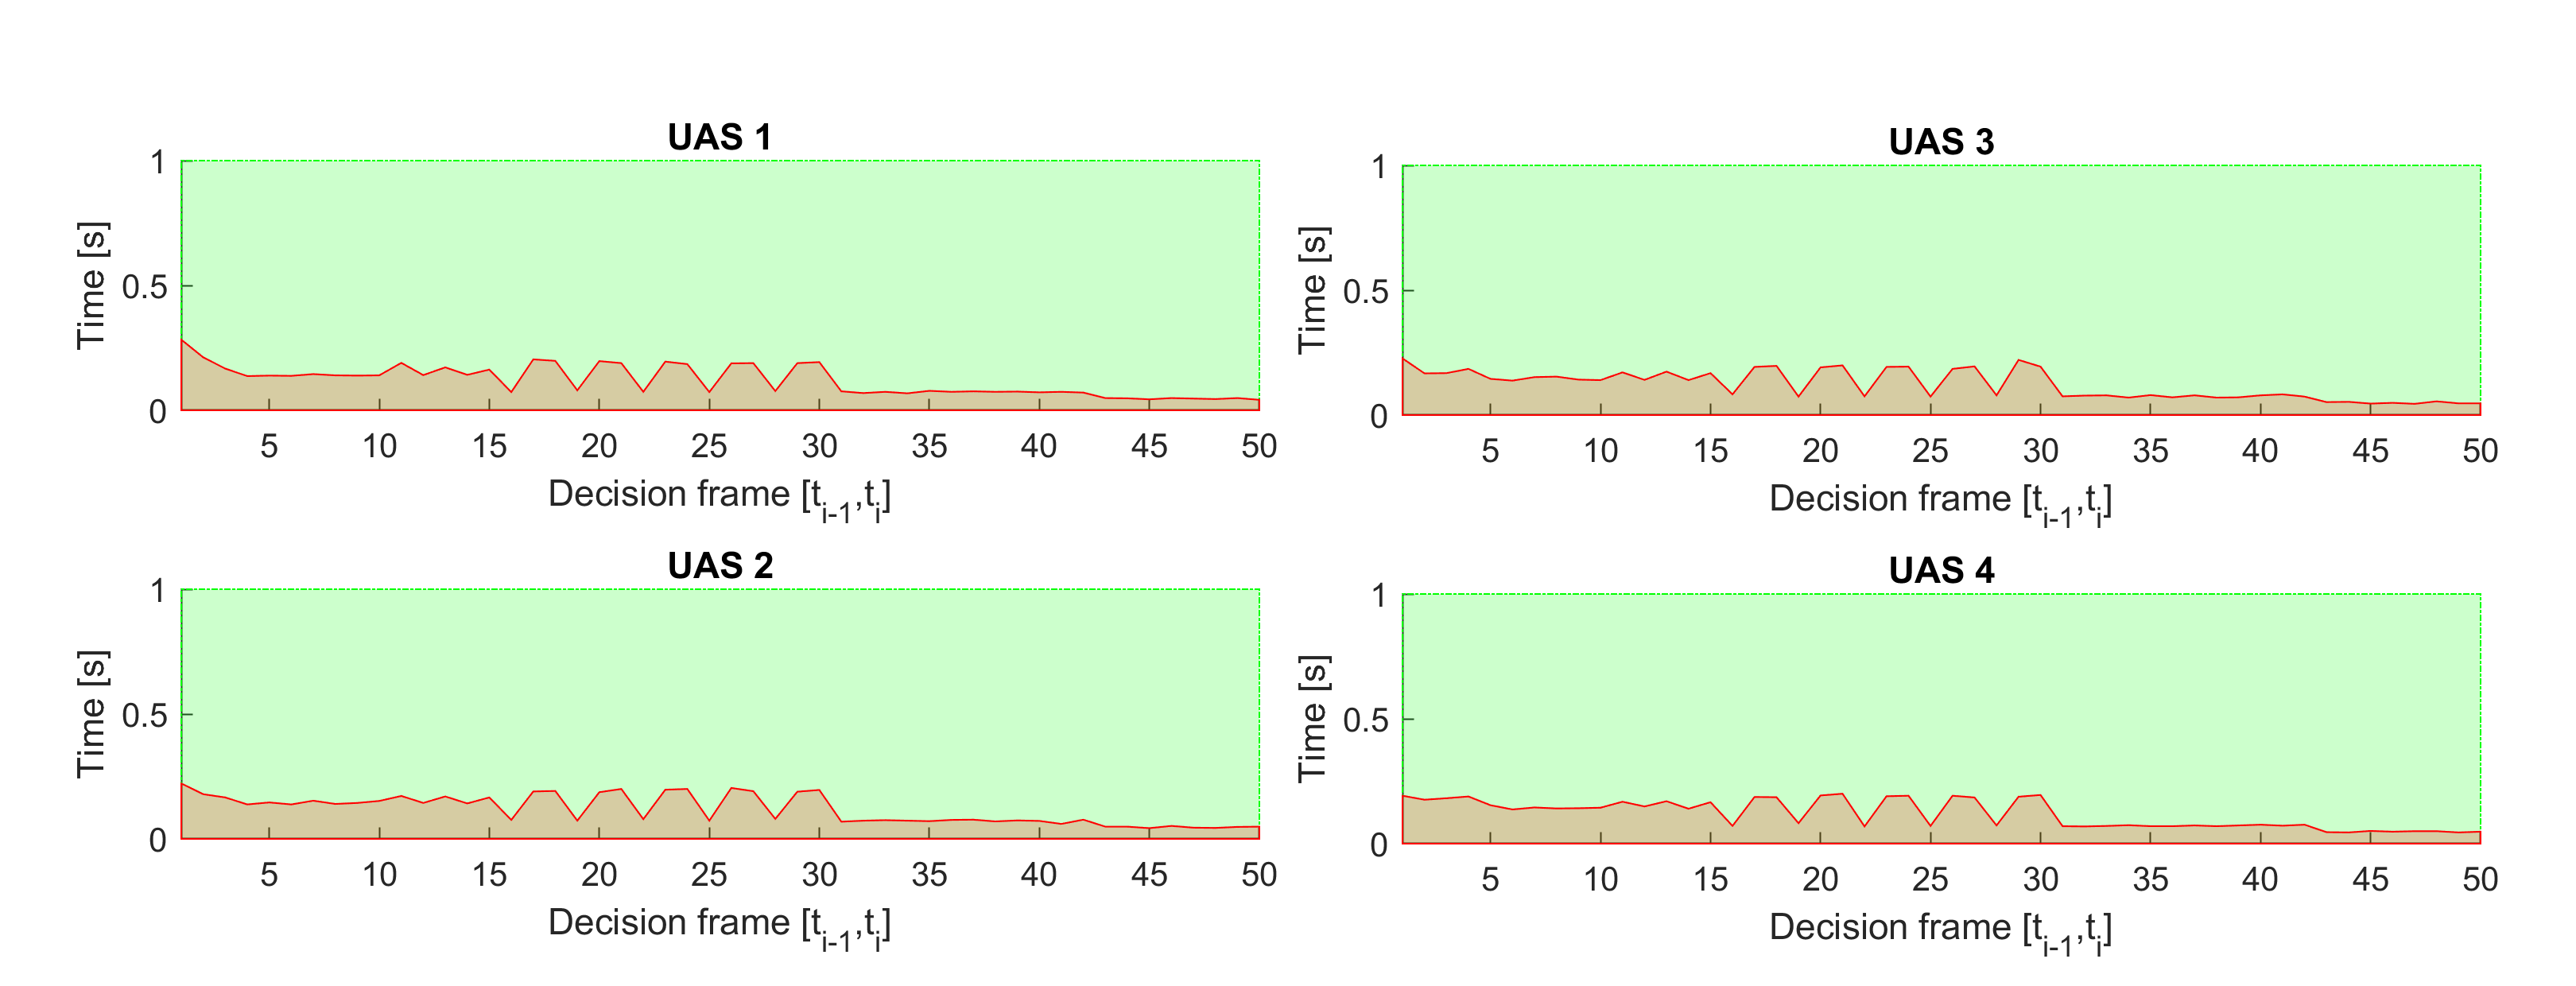
\includegraphics[width=0.95\linewidth]{\FIGDIR/NS101RuleBasedMultipleComputationTime} 
\caption{Computation time for \emph{rule-based multiple} scenario.}
\label{fig:ruleBasedMultipleComputationTime}
\end{figure}